V~této kapitole se ve stručnosti podíváme na základní matematický aparát, se kterým se setkáme v~kvantové mechanice. Klasická mechanika popisuje stav každé částice pomocí šestice proměnných -- tří souřadnic a tří s~ní spojených hybností. Tato šestice vytváří bod v~tzv. fázovém prostoru. Naproti tomu kvantová mechanika popisuje stav systému (např. částice) pomocí vlnové funkce $\psi(x,y,z,t)$, která je funkcí souřadnic a času. Obecně jde o~funkci komplexní, a~proto si nejprve stručně připomeneme základní pravidla práce s~komplexními čísly (viz kapitola \ref{kap:KomplexniCisla}).

V~kvantové mechanice každé měřitelné veličině přiřazujeme operátor. Hodnoty, jichž může měřená veličina nabývat, získáme jako vlastní čísla daného operátoru. Většina úloh v~kvantové mechanice vede na řešení vlastního problému daného operátoru. Proto se seznámíme s~potřebnými partiemi lineární algebry, jako jsou lineární prostor, operátor, vlastní funkce, vlastní číslo atd. (viz kapitola \ref{kap:Operatory}).

\subsection{Komplexní čísla}
\label{kap:KomplexniCisla}

Jako komplexní číslo $Z$ označujeme uspořádanou dvojici reálných čísel $a_1$ a $a_2$. Komplexní číslo $Z = (a_1, a_2)$ nejčastěji zapisujeme v~tzv. algebraickém tvaru $Z = a_1 + i a_2$, kde $i$ je imaginární jednotka, pro kterou platí $i^2 = -1$. Imaginární jednotku definujeme vztahem $i = \sqrt{-1}$. Číslo $a_1$ je reálná část komplexního čísla $Z$, kterou značíme $\mathbf{Re}\, Z$. Číslo $a_2$ je imaginární část komplexního čísla $Z$, kterou značíme $\mathbf{Im} \, Z$. Všechna komplexní čísla $Z$ tvoří množinu komplexních čísel $\mathbb{C}$, proto můžeme psát $Z \in {\mathbb{C}}$.

Z~algebraického tvaru komplexního čísla $Z$ vidíme, že reálná čísla tvoří podmnožinu komplexních čísel a to takových, že pro ně platí $R \equiv Z = a_1 + 0i$, neboli reálné číslo je komplexní číslo ve tvaru $R = (a_1, 0)$. Z~tohoto důvodu platí, že množina reálných čísel $\mathbb{R}$ je podmnožinou komplexních čísel $\mathbb{C}$, což symbolicky zapíšeme jako $\mathbb{R}\subset \mathbb{C}$. Na druhou stranu komplexní číslo, jehož reálná část je rovna nule $J=(0,a_2)$, kde $a_2 \not = 0$ označujeme jako ryze imaginární číslo.

Komplexní čísla můžeme zobrazit jako body v~komplexní rovině, kde kartézskou osu $x$ označujeme jako osu reálných čísel $\mathbf{Re}$ a kartézskou osu $y$ označujeme jako osu ryze imaginární čísel $\mathbf{Im}$ (viz obrázek~\ref{obr:RovinaKomplexnichCisel}).
\begin{figure} [ht]
\centering
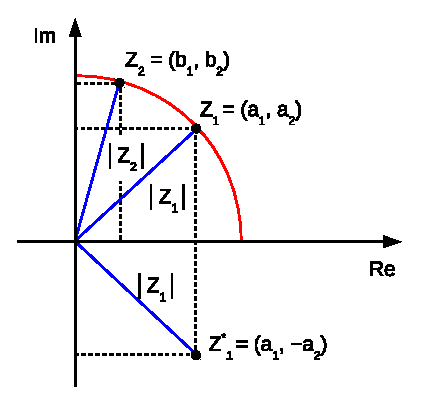
\includegraphics[scale=1]{KomplexniRovina.eps}
\caption[Komplexní rovina]{Znázornění komplexní roviny s~vyznačením komplexních čísel. Dále jsou demonstrovány základní operace s~komplexními čísly -- komplexní sdružení a~absolutní hodnota (modul) komplexního čísla.}
\label{obr:RovinaKomplexnichCisel}
\end{figure}

Protože komplexní čísla tvoří komplexní rovinu, není možné je uspořádat podobně jako reálná čísla. Pro porovnávání komplexních čísel je možné zavést absolutní hodnotu komplexního čísla (modul) vztahem
\begin{equation}
|Z| = \sqrt{a_1^2 + a_2^2} \, \mbox{.}
\label{rov:AbsolutniHodnotaKomplex}
\end{equation}
Absolutní hodnota komplexního čísla je reálné nezáporné číslo a platí, že $|Z| = 0$ právě tehdy, když $Z = 0$. Komplexní čísla, která mají stejnou absolutní hodnotu, leží na kružnici o~poloměru $r = |Z|$ s~počátkem ve středu souřadného systému (v~obrázku \ref{obr:RovinaKomplexnichCisel} vyznačena červeně).

Pro komplexní čísla definujeme stejně jako pro čísla reálná tyto operace: sčítání, odčítání, násobení a dělení. Všechny operace zde pro úplnost shrneme. Mějme dvě komplexní čísla $Z_1 = \nobreak a_1 + ia_2$ a $Z_2=b_1 + ib_2$ zapsaná pro jednoduchost v~algebraickém tvaru.
\begin{enumerate}
\item Při sčítání (odčítání) sčítáme (odčítáme) zvlášť reálnou část a zvlášť imaginární část komplexních čísel.
\begin{equation}
Z_1 \pm Z_2 = (a_1 + ia_2) \pm (b_1 + ib_2) = (a_1 \pm b_1) + i(a_2 \pm b_2)
\label{rov:ScitaniOdcitaniKomplex}
\end{equation}
\item Komplexní čísla násobíme stejně jako dvojčleny. Nesmíme ale zapomenout, že platí vztah $i^2 = -1$.
\begin{equation}
Z_1 \cdot Z_2 = (a_1 + ia_2) \cdot (b_1 + ib_2) = (a_1b_1 - a_2b_2) + i(a_1b_2 + a_2b_1)
\label{rov:NasobeniKomplex}
\end{equation}
\item Dělíme tak, že podíl nejprve rozšíříme vhodnou jedničkou, abychom ve jmenovateli dostali reálné číslo. I~v~oboru komplexních čísel platí, že $b \not = 0$, jinak podíl není definován.
\begin{equation}
\frac{Z_1}{Z_2} = \frac{a_1 + ia_2}{b_1 + ib_2} = \frac{a_1 + ia_2}{b_1 + ib_2} \cdot \frac{b_1 - ib_2}{b_1 - ib_2} = \frac{(a_1b_1 + a_2b_2) + i(a_2b_1 - a_1b_2)}{b_1^2 + b_2^2}
\label{rov:DeleniKomplex}
\end{equation} 
\end{enumerate}

Při počítání s~komplexními čísly je výhodné definovat číslo komplexně sdružené ke komplexnímu číslu $Z$ vztahem
\begin{equation}
Z^\ast = (a_1, a_2)^\ast = (a_1, -a_2) \mbox{,}
\label{rov:KomplexSdruzCislo-uspdvoj}
\end{equation}
nebo podobně v~algebraickém tvaru
\begin{equation}
Z^\ast = (a_1 + ia_2)^\ast = a_1 - ia_2 \mbox{.}
\end{equation}
Geometrická interpretace komplexního sdružení je následující. Komplexně sdružené číslo $Z^\ast$ je osově souměrné ke komplexnímu číslu $Z$ podle osy reálných čísel $\mathbf{Re}$. Na obrázku~\ref{obr:RovinaKomplexnichCisel} je komplexně sdruženo číslo $Z_1$. Vynásobíme-li komplexní číslo s~číslem k~němu komplexně sdruženým, dostaneme kvadrát absolutní hodnoty komplexního čísla, protože
\begin{displaymath}
Z \cdot Z^\ast = (a_1, a_2) \cdot (a_1, a_2)^\ast = (a_1, a_2) \cdot (a_1, -a_2) = (a_1^2 + a_2^2, a_1a_2 - a_1a_2) = (a_1^2 + a_2^2, 0) = |Z|^2 \mbox{,}
\end{displaymath}
\begin{equation}
Z \cdot Z^\ast = |Z|^2 \mbox{.}
\label{rov:KvadradAbsolutniHodnoty}
\end{equation}

Pro sčítání a násobení komplexních čísel platí asociativní, komutativní a distributivní zákon podobně jako u~čísel reálných. Pro komplexně sdružená čísla je možné odvodit následující relace
\begin{equation}
(Z_1 + Z_2)^\ast = Z_1^\ast + Z_2^\ast \mbox{,} \quad (Z_1Z_2)^\ast = Z_1^\ast \cdot Z_2^\ast \mbox{,} \quad \left(\frac{Z_1}{Z_2}\right)^\ast = \frac{Z_2^\ast}{Z_2^\ast} \,\mbox{.}
\label{rov:OperaceSdruzCisla}
\end{equation}

Pro řadu výpočetních aplikací je výhodné komplexní číslo $Z$ zapsat v~tzv. goniometrickém tvaru. Ten odvodíme tak, že v~komplexní rovině zobrazíme komplexní číslo $Z$ a uděláme pravoúhlé průměty absolutní hodnoty komplexního čísla $|Z|$ do reálné $\mathbf{Re}$ a imaginární $\mathbf{Im}$ osy. Označíme-li orientovaný úhel, který svírá průvodič absolutní hodnoty s~osou reálných čísel jako $\theta$, můžeme odvodit, že 
\begin{equation}
a_1 = |Z| \cos \theta \mbox{,} \quad a_2 = |Z| \sin \theta \mbox{.}
\label{rov:PrumetyKomplexnihoCisla}
\end{equation}
Dosadíme-li průměty $a_1$ a $a_2$ z~rovnice (\ref{rov:PrumetyKomplexnihoCisla}) do algebraického tvaru komplexního čísla $Z = a_1 + ia_2$, pak po drobných úpravách odvodíme goniometrický tvar komplexního čísla
\begin{displaymath}
Z = a_1 + ia_2 = |Z| \cos \theta + i (|Z| \sin \theta)
\end{displaymath}
\begin{equation}
Z = |Z| (\cos \theta + i\sin \theta) \mbox{.}
\label{rov:KomplexniCisloGoniomTvar}
\end{equation}
Pro větší názornost je odvození goniometrického tvaru komplexního čísla daného vztahem (\ref{rov:KomplexniCisloGoniomTvar}) graficky znázorněno na obrázku~\ref{obr:GoniometrickyTvar}.
\begin{figure} [ht]
\centering
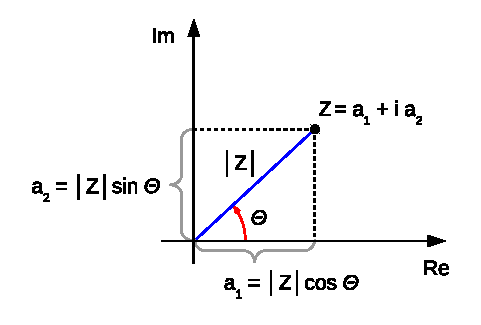
\includegraphics[scale=1]{GoniomTvar.eps}
\caption[Goniometrický tvar komplexního čísla]{K~odvození zápisu komplexního čísla v~goniometrickém tvaru.}
\label{obr:GoniometrickyTvar}
\end{figure}

V~kvantové mechanice se nám bude často hodit tzv. Eulerova identita
\begin{equation}
\boxed{e^{i \theta} = \cos \theta + i \sin \theta \mbox{,}}
\label{rov:EulerovaIdentita}
\end{equation}
která je základem komplexní analýzy, oboru matematiky studujícím funkce komplexní proměnné. Pro zájemce nyní dodáváme její odvození. Nejprve si připomeneme Taylorovu rozvoj funkce $e^{x}$ okolo bodu $x_0 = 0$. Hledaná Taylorova řada je
\begin{equation}
e^x = \sum_{n=0}^{\infty} \frac{x^n}{n!} \,\mbox{.}
\label{rov:TaylorovaRadaExponenciela}
\end{equation}
Pro další použití v~odvození si ještě připomeneme Taylorovy rozvoje funkcí $\sin x$ a $\cos x$
\begin{equation}
\sin x = \sum_{n=0}^{\infty} (-1)^{n} \frac{x^{2n+1}}{(2n+1)!} \mbox{,} \quad \cos x = \sum_{n=0}^{\infty} (-1)^{n} \frac{x^{2n}}{(2n)!} \mbox{.}
\label{rov:RadaCosinusSinus}
\end{equation}
Čistě formální záměnnou $x \equiv i \theta$ ve vztahu (\ref{rov:TaylorovaRadaExponenciela}) dostaneme po rozepsání Taylorovu řadu ve tvaru
\begin{equation}
e^{i\theta} = 1 + i\theta - \frac{\theta^2}{2!} - i \frac{\theta^3}{3!} + \frac{\theta^4}{4!} + i \frac{\theta^5}{5!} -\,\dots
\label{rov:RadaExponenciela1}
\end{equation}
Přeuspořádáním řady (\ref{rov:RadaExponenciela1}) a využitím vztahů (\ref{rov:RadaCosinusSinus}) dostaneme
\newpage
\begin{displaymath}
e^{i\theta} = 1 + i\theta - \frac{\theta^2}{2!} - i \frac{\theta^3}{3!} + \frac{\theta^4}{4!} + i \frac{\theta^5}{5!} -\,\dots =\underbrace{\left(1 - \frac{\theta^2}{2!} + \frac{\theta^4}{4!} - \,\dots \right)}_{\cos \theta} + i \underbrace{\left(x - \frac{\theta^3}{3!} + \frac{\theta^5}{5!} - \,\dots \right)}_{\sin \theta}
\end{displaymath}
\begin{equation}
e^{i\theta} = \cos \theta + i\sin \theta \mbox{,}
\label{rov:DukazEulerovaIdentita}
\end{equation}
což je Eulerova identita, kterou jsme chtěli odvodit. Eulerova identita umožňuje komplexní číslo $Z$ zapsat v~tzv. exponenciálním tvaru.

Exponenciální tvar komplexního čísla $Z$ odvodíme tak, že vyjdeme z~goniometrického tvaru komplexního čísla (\ref{rov:KomplexniCisloGoniomTvar}), do kterého dosadíme Eulerovu identitu (\ref{rov:EulerovaIdentita})
\begin{equation}
Z = |Z| e^{i \theta} \mbox{.}
\label{rov:ExponencialniTvar}
\end{equation}
Exponenciální tvar komplexního čísla je obzvlášť šikovný při násobení a dělení komplexních čísel. Pro násobení komplexních čísel $Z_1 = |Z_1| e^{i \theta}$ a $Z_2 = |Z_2|e^{i \phi}$ v~exponenciálním tvaru dostaneme
\begin{equation}
Z_1Z_2 = |Z_1| \cdot |Z_2| \cdot e^{i(\theta + \phi)} \mbox{.}
\label{rov:NasobeniExponencialniTvar} 
\end{equation}
Podobně pro dělení komplexních čísel $Z_1$ a $Z_2$ dostaneme
\begin{equation}
\frac{Z_1}{Z_2} = \frac{|Z_1|}{|Z_2|} \cdot e^{i(\theta - \phi)} \mbox{.}
\label{rov:DeleniExponencialniTvar}
\end{equation}

Zapíšeme-li komplexní číslo v~exponenciálním tvaru, je intuitivní definovat mocninu komplexního čísla $Z$. Pro počítání s~mocninami platí, že 
\begin{equation}
Z^n = |Z|^n e^{in\theta} \mbox{,}
\label{rov:MocninaKomplexnihoCisla}
\end{equation}
což je hledaná $n$-tá mocnina komplexního čísla $Z$. Dosazením Eulerovy identity (\ref{rov:EulerovaIdentita}) do rovnice (\ref{rov:MocninaKomplexnihoCisla}) můžeme odvodit známou Moivreovu větu
\begin{equation}
(e^{i\theta})^n = e^{i n \theta} \quad \mbox{tj.} \quad (\cos \theta + i \sin \theta )^n = \cos n\theta + i \sin n\theta \mbox{.}
\label{rov:MoivreovaVeta}
\end{equation}

Na závěr kapitoly o~komplexních číslech si ukážeme jeden ilustrační příklad, který demonstruje, jak odvozovat různé goniometrické identity pomocí Moivreovy věty.

\begin{priklad}
\textbf{Zadání:} Odvoďte známé vzorečky pro kosinus a sinus dvojnásobného argumentu
\begin{displaymath}
\cos 2\theta = \cos^2 \theta - \sin^2 \theta \quad \mbox{a} \quad
\sin 2\theta = 2 \sin \theta \cos \theta \mbox{.}
\end{displaymath}
\textbf{Řešení:} Použijeme Moivreovu větu (\ref{rov:MoivreovaVeta}) ve tvaru
\begin{displaymath}
(\cos \theta + i \sin \theta )^2 = \cos^2 \theta + 2 i \cos \theta \sin \theta - \sin^2 \theta = \cos 2 \theta + i \sin 2 \theta
\end{displaymath}
Odtud porovnáním členů s~a bez komplexní jednotky dostaneme vzorečky pro kosinus a sinus dvojnásobného argumentu.
\end{priklad}

\newpage

\subsection{Operátory}
\label{kap:Operatory}

\subsubsection{Co je operátor}

Čtenář je nepochybně intimně seznámen s~pojmem funkce. Funkce představuje matematickou operaci, kdy působením na číslo (nezávisle proměnnou) získáme nové číslo (závisle proměnnou). Operátor naproti tomu představuje matematickou operaci, kdy působením na funkci získáme funkci novou. Působením operátoru $\hat{O}$ na funkci $f$ zapíšeme
\begin{equation}
\boxed{\hat{O} f = g \mbox{,}}
\label{rov:Operator}
\end{equation}
kde výsledkem působení operátoru $\hat{O}$ je nová funkce $g$. Zapamatujme si, že z~definiční rovnice působení operátoru na funkci (\ref{rov:Operator}) plyne, že pořadí operátoru a funkce, na kterou operátor působí, není libovolné, ale že operátor vždy působí na funkci stojící napravo od operátoru.

Abychom se blíže seznámili s~operátory, představme si několik základních typů operátorů. Nejjednodušším operátorem může být operátor
\begin{equation}
\hat{O} = 1,
\nonumber
\end{equation}
neboli operátor identity nebo také jednotkový operátor. Tento operátor působě na libovolnou funkci $f$ vrátí funkci $g$ takovou, že platí $g=1 \cdot f$. Dalším jednoduchým operátorem může být například násobení proměnnou $x$
\begin{equation}
\hat{O} = x.
\nonumber
\end{equation}
Pakliže tento operátor bude působit na funkci $f = x^2$ dostaneme
\begin{equation}
\hat{O} f = x \cdot f = x \cdot x^2 = x^3 = g.
\nonumber
\end{equation}
Další důležitou třídou operátorů jsou diferenciální operátory, například
\begin{equation}
\hat{O} = \frac{\mathrm{d}}{\mathrm{d}x}.
\nonumber
\end{equation}
Vidíme, že derivaci funkce podle proměnné $x$ můžeme chápat jako působení operátoru derivace $\hat{O}$ na funkci $f(x)$. Názorný příklad působení diferenciálního operátoru uvádí příklad \ref{pr:Operator}.

\begin{priklad} \label{pr:Operator}
\textbf{Zadání:} Nalezněte výsledek působení operátoru $\hat{O}=\frac{\mathrm{d}}{\mathrm{d}x}$ na funkci $f(x) = \sin x$. \\
\textbf{Řešení:} Zapíšeme rovnici vyjadřující působení operátoru $\hat{O}$ na funkci $f(x)$ a dostaneme
\begin{displaymath}
\hat{O} f(x) = \frac{\mathrm{d}}{\mathrm{d}x} \sin x = \cos x \equiv g(x)
\end{displaymath}
Vidíme, že výsledkem působení operátoru $\hat{O}$ na funkci $f(x)$ je nová funkce $g(x) = \cos x$.
\end{priklad}

V~kvantové mechanice operátory reprezentující měřitelné veličiny, například pozici, hybnost, moment hybnosti nebo celkovou energii systému. V~kapitole \ref{kap:historie} o~historickém vývoji kvantové mechaniky jsme se seznámili se Schrödingerovou rovnicí popisující pohyb částice v~jedné dimenzi
\begin{equation}
\left( -\frac{\hbar^2}{2m}\frac{\mathrm{d}^2}{\mathrm{d} x^2} + V(x) \right) \Psi(x) = E \Psi(x) \mbox{,}
\label{rov:SCHR}
\end{equation}
Tuto rovnici můžeme přepsat jako operátorovou rovnici, tj. rovnici ve které vystupují operátory
\begin{equation}
\hat{H}\Psi(x) = E \Psi(x)\mbox{,}
\label{rov:SCHR-operator}
\end{equation}
kde $\hat{H}$ je operátor celkové energie systému, tzv. hamiltonián (Hamiltonův operátor). Porovnáním rovnice \eqref{rov:SCHR} s~rovnicí \eqref{rov:SCHR-operator} odvodíme předpis pro hamiltonián
\begin{equation}
\hat{H} \equiv \left( -\frac{\hbar^2}{2m}\frac{\mathrm{d}^2}{\mathrm{d} x^2} + V(x) \right)
\label{rov:Hamiltonian1D}
\end{equation}

V~obecném případě pohybu částice v~třírozměrném prostoru má Hamiltonův operátor tvar
\begin{equation}
\hat{H} \equiv \left( -\frac{\hbar^2}{2m}\Delta + V(x) \right) \mbox{,}
\label{rov:Hamiltonian3D}
\end{equation}
kde symbol $\Delta$ představuje Laplaceův operátor, který je druhou mocninou operátoru nabla $\Delta = \nabla^2$  a v~kartézských souřadnicích má tvar
\begin{equation}
\Delta = \frac{\partial^2}{\partial x^2}+\frac{\partial^2}{\partial y^2}+\frac{\partial^2}{\partial z^2} \mbox{.}
\label{rov:LaplaceuvOperator}
\end{equation}

Konkrétní tvar hamiltoniánu (\ref{rov:Hamiltonian3D}) závisí na konkrétní formě potenciální energie $V(x)$. Například v~případě vodíkového atomu, kdy se elektron pohybuje v~Coulombově poli generovaném protonem bude mít hamiltonián pro elektron tvar
\begin{equation}
\hat{H} \equiv \left( -\frac{\hbar^2}{2m_e}\Delta - \frac{1}{4 \pi \epsilon_0}\frac{e^2}{r} \right) \mbox{,}
\label{rov:HamiltonianVodik}
\end{equation}
kde $e$ je elementární náboj elektronu, $m_e$ je hmotnost elektronu, $\epsilon_0$ je permitivita vakua a $r$ je vzdálenost protonu a elektronu.

Další hojně se vyskytující operátory jsou operátor hybnosti a operátor polohy
\begin{equation}
\hat{p}= -i\hbar \nabla \mbox{,}
\label{rov:OperatorHybnosti}
\end{equation}
\begin{equation}
\hat{r} = \mathbf{r} \mbox{,}
\label{rov:OperatorPozice}
\end{equation}
kde $\mathbf{r}=(x,y,z)$ je polohový vektor v~3D eukleidovském prostoru. Operátory (\ref{rov:OperatorHybnosti}) a (\ref{rov:OperatorPozice}) jsou zapsané v~tzv. souřadnicové reprezentaci, kdy operátor souřadnice je zvolen jako prosté násobení danou souřadnicí.

Vraťme se ještě jednou k~rovnici \eqref{rov:SCHR-operator}, ta je totiž speciálním případem třídy rovnic označovaných jako vlastní problém. Mějme operátor $\hat{O}$ a obecnou funkci $f$, pak rovnice
\begin{equation}
\boxed{\hat{O} f = \lambda f}
\label{rov:VlastniProblem}
\end{equation}
se označuje jako \textbf{vlastní problém operátoru} $\hat{O}$. Funkci $f$ pak nazýváme \textbf{vlastní funkce} operátoru $\hat{O}$ s~vlastním číslem $\lambda$. Jinak řečeno vlastní funkce $f$ operátoru $\hat{O}$ je taková funkce, že působí-li na ni operátor $\hat{O}$, pak výsledkem tohoto působení je funkce $f$ vynásobená číslem $\lambda$. V~případě rovnice \eqref{rov:SCHR-operator} je vlastní funkcí operátoru $\hat{H}$ vlnová funkce $\Psi(x)$ s~vlastním číslem $E$, celková energie systému. Vlastní problém operátoru má ústřední postavení v~kvantové mechanice, protože řešení většiny úloh znamená hledání vlastních čísel a vlastních funkcí příslušného operátoru. 



\subsubsection{Operace s~operátory}
\label{kap:OperaceSOperatory}

Podobně jako funkce můžeme mezi sebou sčítat, násobit, dělit atd. definujeme tyto operace i~pro počítání s~operátory. Vyjdeme ze vztahu (\ref{rov:Operator}), který definuje působení operátoru na funkci $f$ a ve stručnosti si představíme základní operace s~operátory.

Součtem dvou operátorů budeme rozumět operátor
\begin{equation}
\hat{C} = \hat{A}+\hat{B}
\label{rov:SoucetOperatoru1}
\end{equation}
takový, že platí
\begin{equation}
\hat{C}f = (\hat{A}+\hat{B})f=\hat{A}f + \hat{B}f \mbox{,}
\label{rov:SoucetOperatoru2}
\end{equation}
kde $f$ je libovolná testovací funkce. Pod součinem operátorů budeme rozumět operátor
\begin{equation}
\hat{C} = \hat{A}\hat{B}
\label{rov:SoucinOperatoru1}
\end{equation}
takový, že platí
\begin{equation}
\hat{C}f = \hat{A}(\hat{B}f) \mbox{.}
\label{rov:SoucinOperatoru2}
\end{equation}
Stejně jako v~případě násobení čísel figuruje číslo $1$ jako jednotkový prvek vůči násobení, je i~v~případě operátorového počtu definován jednotkový prvek -- jednotkový operátor $\hat{1}$
\begin{equation}
\hat{1} f = f \mbox{.}
\label{rov:JednotkovyOperator}
\end{equation}

\noindent Pomocí definice násobení operátorů (\ref{rov:SoucinOperatoru1}) můžeme definovat druhá mocnina operátoru
\begin{equation}
\hat{A}^2 = \hat{A}\hat{A} \mbox{.}
\label{rov:KvadratOperatoru} 
\end{equation}
A~dále matematickou indukcí můžeme definovat $n$-tou mocninu operátoru
\begin{equation}
\hat{A}^n f = \hat{A} (\hat{A}^{n-1} f) \mbox{.}
\label{rov:MocninaOperatoru}
\end{equation}

Obecně platí, že násobení operátorů (\ref{rov:SoucinOperatoru1}) není komutativní, to znamená, že neplatí
\begin{equation}
\hat{A}\hat{B} = \hat{B}\hat{A} \mbox{.}
\label{rov:KomutativnostOperatoru}
\end{equation}
Abychom mohli vyšetřovat komutativnost operátorů, zavádí se nový operátor -- \textbf{komutátor}
\begin{equation}
\boxed{[\hat{A},\hat{B}] \equiv \hat{A}\hat{B}-\hat{B}\hat{A} \mbox{.}}
\label{rov:KomutatorOperatoru}
\end{equation}
Když je komutátor dvou operátorů roven nulovému operátoru ($\hat{0}f=0$)
\begin{equation}
[\hat{A},\hat{B}] = \hat{0} \mbox{,}
\label{rov:Komutator1}
\end{equation}
říkáme, že operátory $\hat{A}$ a $\hat{B}$ spolu komutují. Když se komutátor nerovná nulovému operátoru, operátory nekomutují.

Jako příklad vyšetřování komutátoru dvou operátorů si spočtěme komutátor mezi operátorem hybnosti \eqref{rov:OperatorHybnosti} a souřadnice \eqref{rov:OperatorPozice}. Dostaneme
\begin{equation}
[\hat{r},\hat{p}] = -i \hbar \mathbf{r} \nabla + i \hbar \nabla \mathbf{r} = i \hbar (\nabla \mathbf{r} - \mathbf{r} \nabla) = i \hbar,
\nonumber
\end{equation}
kde jsme využili identity z~vektorové analýzy $\nabla \mathbf{r} - \mathbf{r} \nabla = \hat{1}$. Abychom ukázali, že tato identita platí, představme si, že řešíme problém pouze v~jedné dimenzi a současně si povšimněme, že levá strana identity má tvar komutátoru dvou operátorů. Dále víme, že komutátor je také operátor, který můžeme nechat působit na libovolnou funkci $f$. Dostaneme
\begin{equation}
\frac{\partial x f}{\partial x} - x\frac{\partial f}{\partial x} = f + xf^{\prime} - xf^{\prime} = f,
\nonumber
\end{equation}
kde první derivace je derivací součinu dvou funkcí. Odstraněním testovací funkce $f$ dostaneme
\begin{equation}
\frac{\partial x }{\partial x} - x\frac{\partial }{\partial x} = \hat{1},
\nonumber
\end{equation}
což je vektorová identita, kterou jsme chtěli dokázat.

Jak jsme ukázali v~názorném příkladu, výsledkem komutátoru operátoru momentu hybnosti a souřadnice je operátor
\begin{equation}
\boxed{[\hat{r},\hat{p}] = i \hbar,}
\label{rov:KomutatorHybnostSouradnice}
\end{equation}
který se nerovná nulovému operátoru, proto můžeme shrnout, že operátor hybnosti nekomutuje s~operátorem souřadnice.

\begin{priklad} \label{pr:Komutator}
\textbf{Zadání:} Určete komutátor operátorů $\hat{A} = \partial/\partial x$ a $\hat{B} = \partial / \partial y$. \\
\textbf{Řešení:} Sestavíme komutátor $[\hat{A},\hat{B}]$ a necháme ho působit na testovací funkci $f=f(x,y)$. Dostaneme
\begin{displaymath}
[\hat{A},\hat{B}] f = \frac{\partial f}{\partial x} \frac{\partial f}{\partial y} - \frac{\partial f}{\partial y} \frac{\partial f}{\partial x} = \frac{\partial^2 f}{\partial x \partial y} - \frac{\partial^2 f}{\partial y \partial x} = \hat{0},
\end{displaymath}
kde poslední rovnost je splněna tehdy, když funkce $f$ má spojité všechny druhé parciální derivace.

Vidíme, že výsledkem působení komutátoru je nulový operátor, proto můžeme uzavřít, že operátory $\hat{A}$ a $\hat{B}$ spolu komutují.
\end{priklad}

Z~definice komutátoru (\ref{rov:KomutatorOperatoru}) vyplývají tři důležité vlastnosti komutátorů. První vlastností je \textbf{antisymetrie}
\begin{equation}
[\hat{A},\hat{B}] = -[\hat{B},\hat{A}],
\label{rov:VlastnostKomutatoru1}
\end{equation}
která se týká toho, že záleží na pořadí operátorů v~komutátoru. To souvisí s~tím, že operátory obecně nekomutují. Například platí
\begin{equation}
[\hat{r},\hat{p}]= i \hbar,
\nonumber
\end{equation}
ale
\begin{equation}
[\hat{p},\hat{r}]= - i \hbar.
\nonumber
\end{equation}
Druhou vlastností je \textbf{linearita} v~druhém argumentu
\begin{equation}
[\hat{A},\hat{B}+\hat{C}] = [\hat{A},\hat{B}] + [\hat{A},\hat{C}].
\label{rov:VlastnostKomutatoru2}
\end{equation}
Ta souvisí s~tím, že komutátor je lineární operátor (viz další kapitola \ref{kap:OperatorySpecifickychVlastnosti}). Třetí vlastnost
\begin{equation}
[\alpha \cdot \hat{A},\hat{B}] = \alpha \cdot [\hat{A},\hat{B}]
\label{rov:VlastnostKomutatoru3}
\end{equation}
souvisí s~tím, že číslo $\alpha$ můžeme z~komutátoru vytknout.

Na závěr této kapitoly uvedeme jedno důležité tvrzení. \textbf{Komutují-li spolu dva operátory, tj. $[\hat{A},\hat{B}]=\hat{0}$, pak nutně mají společné vlastní funkce $f$.} Tvrzení si dokážeme. Předpokládejme, že máme dva libovolné operátory $\hat{A}$ a $\hat{B}$, pro které platí
\begin{equation}
\hat{A} f = a f
\nonumber
\end{equation}
a
\begin{equation}
\hat{B} f = b f,
\nonumber
\end{equation}
neboli operátory mají stejnou vlastní funkci $f$. Pak můžeme psát
\begin{equation}
\hat{A}\hat{B} f = \hat{A} (b f) = a b f
\nonumber
\end{equation}
a 
\begin{equation}
\hat{B}\hat{A} f = \hat{B} (a f) = a b f,
\nonumber
\end{equation}
protože čísla $a$ a $b$ komutují vždy. Odečtením předchozích dvou rovnic dostaneme
\begin{equation}
\hat{A}\hat{B} f - \hat{B}\hat{A} f  = (\hat{A}\hat{B} - \hat{B}\hat{A} ) f = [\hat{A}, \hat{B}] f = 0,
\nonumber
\end{equation}
což je výsledek, který jsme chtěli ukázat. Důkaz tvrzení je tak proveden. \hfill {\footnotesize $\blacksquare$}

\subsubsection{Prostory funkcí a Hilbertův prostor}
\label{kap:ProstoryFunkci}

Matematické objekty jako funkce nebo operátory jsou definovány na určitém prostoru $\mathcal{V}$. Prostor je v~matematice definován jako množina prvků, s~kterými je možné provádět jisté operace. Ze základního kurzu matematiky znáte lineární vektorový prostor $\mathcal{V}$ s~dvěma operacemi, sčítáním $+$ a násobením číslem $\cdot$, kde prvky prostoru jsou vektory, neboli uspořádané $N$-tice čísel.

Omezme se nyní v~našich úvahách na lineární vektorový prostor $\mathbb{R}^3$, který můžeme chápat jako 3D eukleidovský prostor. Pak libovolný vektor $\mathbf{v} = (v_1, v_2, v_3)$ můžeme pravoúhle promítnout do tří souřadných os, neboli reprezentovat tento vektor pomocí souboru vektorů souřadných os $e_1 = (1, 0, 0)$, $e_2 = (0, 1, 0)$ a $e_3 = (0, 0, 1)$.

Abychom nalezli tuto reprezentaci, tj. byli schopni vektor $\mathbf{v}$ zapsat pomocí vektorů souřadných os, nejprve určíme velikost průmětu vektoru $\mathbf{v}$ do jednotlivých souřadných os. K~tomu nám poslouží skalární součin vektoru $\mathbf{v}$ s~vektory souřadných os
\begin{equation}
\braket{e_i|\mathbf{v}} = v_i,
\nonumber
\end{equation}
kde zvolená symbolika pro skalární součin má své opodstatnění, jak uvidíme později. Vektor $\mathbf{v}$ tak můžeme v~reprezentaci vektorů souřadných os zapsat jako
\begin{equation}
\mathbf{v} = \sum_{i=1}^{3} \braket{e_i|\mathbf{v}} e_i.
\label{rov:RozvojVektoruDoBaze}
\end{equation}
Vztah \eqref{rov:RozvojVektoruDoBaze} si zaslouží pár poznámek. Zaprvé si uvědomme, že výsledkem skalárního součinu $\braket{e_i|\mathbf{v}}$ je číslo. Za druhé vektor je prvek mající velikost i směr, ve vztahu \eqref{rov:RozvojVektoruDoBaze} se o~velikost \uv{stará} skalární součin a o~směr jednotkové vektory souřadných os.

Vidíme, že abychom vektor $\mathbf{v}$ \uv{zrekonstruovali} z~vektorů reprezentující osy souřadného systému, musí být tento soubor vektorů $\{e_i\}$ úplný. Tak například, kdyby chyběl vektor $e_2$, nikdy bychom nebyli schopni zreprodukovat složku $v_2$ vektoru $\mathbf{v}$. Došli jsme k~závěru, že úplný soubor vektorů $\{e_i\}$ umožňuje reprezentovat libovolný prvek z~daného prostoru.

Úplný soubor vektorů $\{e_i\}$ bývá zvykem označovat za bázi daného prostoru. Báze má několik základních vlastností:
\begin{enumerate}
\item počet prvků báze je roven dimenzi prostoru,
\item pro libovolné dva prvky báze platí $\braket{e_i|e_j} = 0$, tj. prvky jsou na sebe kolmé -- ortogonální.
\end{enumerate}

Obeznámeni s~lineárními vektorovými prostory můžeme přistoupit k~definici prostoru funkcí. Prostor funkcí je prostor prvků, kterými jsou funkce mající jisté vlastnosti. V~analogii s~vektorovými prostory i zde existuje úplný soubor funkcí, do kterého můžeme rozložit libovolnou funkci prostoru
\begin{equation}
f = \sum_i c_i \varphi_i,
\label{rov:RozvojDoBazeFunkci}
\end{equation}
kde funkce $\varphi_i$ tvoří úplný soubor funkcí $\{\varphi_i\}$ a $c_i$ jsou rozvojové koeficienty. Příkladem úplného souboru funkcí je například soubor $x, x^2, x^3, \dots, x^n$.

V~kvantové mechanice je ústředním funkčním prostorem Hilbertův prostor, jehož prvky jsou kvadraticky integrovatelné komplexní funkce  splňující
\begin{equation}
\boxed{\int_{-\infty}^{\infty} |f(x)|^2 \,\mathrm{d}x < \infty}
\label{rov:KvandarickaIntegrovatelnost}
\end{equation} 
a dále je na tomto prostoru definována další vlastnost, skalární součin dvou funkcí
\begin{equation}
\boxed{\braket{f|g} \equiv \int_{-\infty}^{\infty} f^{\ast}(x) g(x) \mathrm{d}x,}
\label{rov:SkalarniSoucinFci}
\end{equation}
kde $^{\ast}$ značí komplexně sdruženou funkci. Zápis skalárního součinu ve tvaru $\braket{f|g}$, kde symbol $\bra{f}$ označovaný jako bra-vektor znamená komplexně sdruženou funkci $f^{\ast}$, symbol $\ket{g}$ označovaný jako ket-vektor znamená funkci $g$ a celý uzavřený symbol neboli braket chápeme jako integraci součinu funkcí $f^{\ast}g$, pochází od britského teoretického fyzika P.\,A.\,M.\,Diraca. Tato tzv. braketová notace se v~kvantové mechanice hojně využívá pro svou eleganci a úsporné zkrácení zápisu, který by byl jinak velmi složitý. V našem textu se této notaci spíše vyhýbáme.



\subsubsection{Operátory specifických vlastností}
\label{kap:OperatorySpecifickychVlastnosti}

Kvantová mechanika pracuje výhradně s~lineárními operátory, aby byl splněn princip superpozice, tj. jsou-li $\psi_1$ a $\psi_2$ vlnové funkce daného systému, pak i funkce $\psi=c_1\psi_1+c_2\psi_2$, kde $c_1$ a $c_2$ jsou libovolná komplexní čísla, je vlnovou funkcí uvažovaného systému. Pro lineární operátory platí
\begin{equation}
\boxed{\hat{A} (\alpha f + \beta g) = \alpha\hat{A}f + \beta\hat{A}g \mbox{,}}
\label{rov:LinearitaOperatoru}
\end{equation}
kde $\alpha$ a $\beta$ jsou obecně komplexní čísla.

Nejdůležitější operátory kvantové mechaniky jsou tzv. Hermitovy operátory $\hat{H}$ definované tak, že působí stejně na obou stranách skalárního součinu \eqref{rov:SkalarniSoucinFci}
\begin{equation}
\boxed{\int f^{\ast} \hat{H} g \,\mathrm{d}x = \int g \hat{H}^{\ast} f^{\ast} \,\mathrm{d}x,}
\label{rov:DefiniceHermitovaOperatoru}
\end{equation}
což můžeme v~braketové notaci zapsat jako
\begin{equation}
\braket{\hat{H}f|g} = \braket{f|\hat{H}g} \mbox{.}
\nonumber
\end{equation}
Z~definiční rovnice \eqref{rov:DefiniceHermitovaOperatoru} Hermitova operátoru vyplývá, že
\begin{equation}
\hat{H}^{\ast} = \hat{H} \mbox{.}
\nonumber
\end{equation}
Skutečnost, že Hermitovy operátory působí stejně v~levé i v~pravé straně skalárního součinu, se často značí následovně
\begin{equation}
\braket{f|\hat{H}|g} \mbox{.}
\nonumber
\end{equation}
Centrální pozice Hermitova operátoru $\hat{H}$ říká, že je jen na nás, zda necháme operátor působit v~levé nebo pravé straně skalárního součinu.

Nyní se podíváme na několik základních vlastností hermitovských operátorů. První vlastností je, že vlastní čísla hermitovského operátoru jsou reálná
\begin{equation}
\boxed{h^\ast = h.}
\label{rov:RealnaVlastniCisla}
\end{equation}
Tuto vlastnost si dokážeme. Uvažujme vlastní problém hermitovského operátoru
\begin{equation}
\hat{H} \psi = h \psi.
\nonumber
\end{equation}
Postupujme tak, že nejprve vlastní problém komplexně sdružíme
\begin{equation}
\hat{H}^\ast \psi^\ast = h^\ast \psi^\ast.
\nonumber
\end{equation}
Nyní vynásobme zleva komplexně sdružený vlastní problém funkcí $\psi$ a vlastní problém funkcí $\psi^\ast$ a integrujme, dostaneme
\begin{equation}
\int \psi \hat{H}^\ast \psi^\ast \,\mathrm{d}x = h^\ast \int \psi \psi^\ast \,\mathrm{d}x  = h^\ast
\nonumber 
\end{equation}
a
\begin{equation}
\int \psi^\ast \hat{H} \psi \,\mathrm{d}x = h \int \psi^\ast \psi \,\mathrm{d}x  = h.
\nonumber 
\end{equation}
Protože je operátor $\hat{H}$ hermitovský, platí
\begin{equation}
\int \psi \hat{H}^\ast \psi^\ast \,\mathrm{d}x = \int \psi^\ast \hat{H} \psi \,\mathrm{d}x
\nonumber
\end{equation}
a po odečtení posledních rovnic dostaneme
\begin{equation}
\int \psi \hat{H}^\ast \psi^\ast \,\mathrm{d}x - \int \psi^\ast \hat{H} \psi \,\mathrm{d}x =0  = h^\ast - h,
\nonumber
\end{equation}
a tedy
\begin{equation}
h^\ast = h,
\nonumber
\end{equation}
což jsme chtěli dokázat. \hfill {\footnotesize $\blacksquare$}

Dále ukážeme, že vlastní funkce hermitovského operátoru příslušející různým vlastním číslům jsou ortogonální, tj.
\begin{equation}
\boxed{\int_{-\infty}^{\infty} f_j^\ast f_i \,\mathrm{d}x = \delta_{ij},}
\label{rov:OrtogonalniVlastniFunkce}
\end{equation}
kde symbol $\delta_{ij}$ značí Kroneckerovo delta, které nabývá hodnoty $1$, když $i=j$ a hodnoty $0$, když $i \not = j$. Pomocí braketové symboliky můžeme vztah \eqref{rov:OrtogonalniVlastniFunkce} zapsat ve tvaru
\begin{equation}
\braket{f_i|f_j} = \delta_{ij}.
\nonumber
\end{equation}
Opět si tvrzení dokážeme. Předpokládejme platnost vztahů
\begin{equation}
\hat{H} \psi_1 = h_1 \psi_1
\nonumber
\end{equation}
a
\begin{equation}
\hat{H} \psi_2 = h_2 \psi_2 \mbox{,}
\nonumber
\end{equation}
kde $h_1 \not = h_2$. První rovnici vynásobíme zleva $\psi_2^\ast$ a integrujeme, druhou rovnici vynásobíme zleva $\psi_1^\ast$ a integrujeme, dostaneme
\begin{equation}
\int \psi_2^\ast \hat{H} \psi_1 \,\mathrm{d}x  = h_1 \int \psi_2^\ast \psi_1 \,\mathrm{d}x
\nonumber
\end{equation}
a
\begin{equation}
\int \psi_1^\ast \hat{H} \psi_2 \,\mathrm{d}x  = h_2 \int \psi_1^\ast \psi_2 \,\mathrm{d}x.
\nonumber
\end{equation}
Dále komplexně sdružíme například první rovnici a rovnice odečteme
\begin{equation}
0 = (h_1 - h_2 ) \int \psi_1^\ast \psi_2 \,\mathrm{d}x.
\nonumber
\end{equation}
Při úpravách jsme využili toho, že operátor $\hat{H}$ je hermitovský a že hermitovské operátory mají reálná vlastní čísla. Protože podle našeho počátečního předpokladu platí $h_1 \not = h_2$ je zřejmé, že musí platit
\begin{equation}
\int \psi_1^\ast \psi_2 \,\mathrm{d}x = 0,
\nonumber
\end{equation}
což jsme chtěli ukázat. Důkaz je tak proveden. \hfill {\footnotesize $\blacksquare$}

Na závěr si uveďme bez důkazu poslední důležitou vlastnost hermitovských operátorů. Soubor vlastních funkcí hermitovského operátoru vytváří úplný soubor bázových funkcí daného Hilbertova prostoru. To znamená, že když platí
\begin{equation}
\hat{H} f_i = h_i f_i \quad \mbox{pro každé}\quad i,
\nonumber
\end{equation}
pak libovolnou funkci $\psi$, můžeme zapsat jako lineární kombinaci
\begin{equation}
\psi = \sum_{i} c_i f_i,
\nonumber
\end{equation}
kde $c_i$ jsou rozvojové koeficienty.



\subsubsection{Postuláty kvantové mechaniky a operátory}
\label{kap:PostulatyKvantoveMechaniky}

Kvantová mechanika, podobně jako klasická Newtonova mechanika, je založena na několika postulátech shrnutých v~kapitole \ref{kap:historie}. Obsahem druhého postulátu je tvrzení, že \textbf{každé fyzikální veličině, kterou můžeme pro danou částici naměřit, je přiřazen operátor, který působí na vlnovou funkci.} Přitom se předpokládá, že operátor je lineární a hermitovský. Hermicita operátoru je nezbytná z~hlediska měření fyzikálních veličin, protože podle třetího postulátu \textbf{jediné hodnoty, které může měřitelná fyzikální veličina $A$ při jednotlivých měřeních nabývat, jsou vlastní čísla $a_n$ odpovídajícího operátoru $\hat{A}$.}

Obsahem čtvrtého postulátu je střední hodnota měření veličiny $A$ na kvantově mechanickém souboru. \textbf{Je-li systém popsán v~okamžiku měření normovanou vlnovou funkcí $\psi$, pak výsledkem měření na odpovídajícím kvantově mechanickém souboru je střední hodnota veličiny $A$ daná vztahem}
\begin{equation}
\boxed{\bar{A} = \int \psi^\ast \hat{A} \psi \,\mathrm{d}x,}
\label{rov:StředniHodnotaVeliciny}
\end{equation}
kde integrace se provádí přes celý dostupný prostor. V~duchu braketové notace můžeme psát
\begin{equation}
\bar{A} = \braket{\psi|\hat{A}|\psi} \mbox{.}
\nonumber
\end{equation}

Jestliže vlnová funkce $\psi$ je vlastní funkcí hermitovského operátoru $\hat{A}$ s~vlastním číslem $a$~pak
\begin{equation}
\bar{A} = \int \psi^{\ast} \hat{A} \psi \,\mathrm{d}x = \int \psi^{\ast} a \psi \,\mathrm{d}x = a \int \psi^{\ast} \psi \,\mathrm{d}x.
\label{rov:MerenaHodnota1}
\end{equation}
Výsledek (\ref{rov:MerenaHodnota1}) můžeme interpretovat následovně. Připravíme-li systém tak, že je charakterizovaný vlnovou funkcí, která je vlastní funkcí příslušného operátoru $\hat{A}$, poskytne opakované měření veličiny příslušné k~operátoru $\hat{A}$ vždy stejnou hodnotu fyzikální veličiny -- vlastní číslo~$a$.

V~případě, že se nám nepodaří systém připravit tak, aby byl charakterizovaný vlastní funkcí příslušného operátoru, můžeme vlnovou funkci systému rozvinout do báze příslušného prostoru. Nechť $\psi$ je obecná vlnová funkce popisující systém. Vlnovou funkci $\psi$ můžeme rozvinout do vlastních funkcí daného hermitovského operátoru $\psi=\sum c_n \phi_n$, kde $\hat{A}\phi_n = a_n \phi_n$, které tvoří úplný soubor na daném Hilbertově prostoru. Pak pro střední hodnotu platí
\begin{eqnarray}
&\bar{A}&=\braket{\psi|\hat{A}|\psi}= \braket{\sum_m c_m \phi_m|\hat{A}|\sum_n c_n \phi_n}=\sum_{m,n} c_m^\ast c_n \braket{\phi_m|\hat{A}\phi_n} {}
\nonumber\\
& & {}= \sum_{m,n} c_m^\ast c_n \braket{\phi_m|a_n \phi_n} = \sum_{m,n} c_m^\ast c_n a_n \braket{\phi_m|\phi_n} \mbox{.}
\label{rov:MerenaHodnota2}
\end{eqnarray}
Protože vlastní funkce hermitovského operátoru jsou ortogonální (viz vztah \eqref{rov:OrtogonalniVlastniFunkce}) je skalární součin ve výrazu (\ref{rov:MerenaHodnota2}) nenulový pouze když $m=n$. Proto se dvojitá suma zredukuje na jednoduchou a výraz (\ref{rov:MerenaHodnota2}) přejde na jednoduchý tvar
\begin{equation}
\bar{A} = \sum_n c_n^\ast c_n a_n = \sum_n |c_n|^2 a_n \mbox{.}
\label{rov:MerenaHodnota3}
\end{equation}
Všimněme si výsledku, který jsme obdrželi. Střední hodnota veličiny na souboru popsaném vlnovou funkcí $\psi=\sum c_n \phi_n$ se počítá jako vážená suma vlastních čísel daného operátoru. Váhami jsou v~tomto případě kvadráty rozvojových koeficientů $|c_n|^2$, které mají význam pravděpodobnosti, že při měření na souboru naměříme právě hodnotu $a_n$.

Je to vztah (\ref{rov:MerenaHodnota3}), který z~kvantové mechaniky dělá pravděpodobnostní teorii. Protože pouze tehdy, když systém připravíme ve stavu, který odpovídá vlastní funkci příslušného operátoru, dostaneme při opakovaném měření té samé veličiny stejný výsledek, přesně podle vztahu (\ref{rov:MerenaHodnota1}). Ve všech ostatních případech můžeme pouze určit pravděpodobnost toho, že změříme danou hodnotu veličiny, která je určená kvadrátem rozvojových koeficientů vlnové funkce popisující systém do báze vlastních funkcí hermitovského operátoru.


\subsubsection{Maticová reprezentace operátorů}


Zabývejme se ještě na chvíli rozvojem libovolné funkce do báze daného prostoru, který je dán vztahem \eqref{rov:RozvojDoBazeFunkci}. A~pro jednoduchost zápisu adoptujme pro tuto chvíli braketovou notaci. Potom obecnou funkci $\ket{\psi}$ můžeme rozvinout do úplného souboru funkcí $\ket{\varphi_i}$
\begin{equation}
\ket{\psi} = \sum_i c_i \ket{\varphi_i} \mbox{.}
\nonumber
\end{equation}
Pak pro vlastní problém $\hat{A} \ket{\psi} = a \ket{\psi}$ můžeme psát
\begin{equation}
\sum_i c_i \hat{A} \ket{\varphi_i} = a \sum_i c_i \ket{\varphi_i} \mbox{.}
\nonumber
\end{equation}
Rovnici vynásobme zleva jednou konkrétní funkcí z~úplného souboru funkcí, například funkcí $\bra{\varphi_m}$
\begin{equation}
\sum_i c_i \braket{\varphi_m|\hat{A}|\varphi_i} = a \sum_i c_i \braket{\varphi_m|\varphi_i}= a c_m \mbox{,}
\label{rov:Matice4}
\end{equation}
kde jsme využili toho, že úplný soubor funkcí jsou vlastní funkce hermitovského operátoru, které jsou ortogonální, tj. skalární součin $\braket{s_m|s_i}$ je nenulový jenom v~případě, kdy $m=i$. Výsledkem je, že v~sumaci na pravé straně výrazu (\ref{rov:Matice4}) zůstane nenulový jen člen $a c_m$. Dále provedeme substituci
\begin{equation}
A_{mi} \equiv \braket{\varphi_m|\hat{A}|\varphi_i} \mbox{,}
\nonumber
\end{equation}
kde výraz $A_{mi}$ označujeme jako maticový element. Výsledkem je 
\begin{equation}
\sum_i A_{mi} \, c_i = a c_m \mbox{.}
\label{rov:Matice6}
\end{equation}
Rovnici (\ref{rov:Matice6}) můžeme zapsat pro $\forall m$ a výslednou soustavu $m$-rovnic zapíšeme jako maticovou rovnici
\begin{equation}
\boxed{\mathbb{A} \mathbf{c} = a \mathbf{c} \mbox{,}}
\label{rov:Matice7-vysledek}
\end{equation}
kde $\mathbb{A}$ je čtvercová matice $(m \times i)$ a $\mathbf{c}$ je sloupcový vektor rozvojových koeficientů.

Došli jsme k~důležitému závěru, který si zasluhuje bližší komentář. Pomocí postupu uvedeného výše jsme došli k~tomu, že řešení vlastního problému operátoru $\hat{A}$ se redukuje na počítání s~maticemi. Vzhledem k~tomu, že násobení matic je obecně nekomutativní, mají matice příhodné vlastnosti, aby byly vhodnou reprezentací operátorů. Toho si povšiml jako první německý fyzik Werner Heisenberg a formuloval svou interpretaci kvantové mechaniky, která vešla ve známost jako maticová mechanika.








